\documentclass[border=2mm]{standalone}
\usepackage{tikz}
\usetikzlibrary{arrows,shapes,snakes,automata,backgrounds,petri,matrix}

\begin{document}
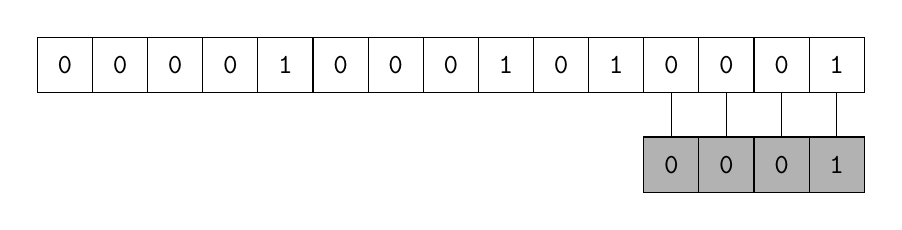
\begin{tikzpicture}[
font=\ttfamily, array/.style={
    matrix of nodes, 
    nodes={draw=black, minimum size=7mm, fill=white, anchor=center},
    column sep=-\pgflinewidth, 
    row sep=5.5mm, 
    row 1/.style={ nodes={draw=black, fill=none, minimum size=7mm}},
    row 1 column 1/.style={nodes={draw}},
},
]

\matrix[array] (array) {
   0  &  0  &  0  &  0  &  1  & 0 & 0 & 0 & 1 & 0 & 1 & 0 & 0 & 0 & 1\\
  &&&&&&&&&&& |[fill=gray!60]|0 & |[fill=gray!60]|0 & |[fill=gray!60]| 0 & |[fill=gray!60]|1 \\
};

\draw (array-1-12) to (array-2-12);
\draw (array-1-13) to (array-2-13);
\draw (array-1-14) to (array-2-14);
\draw (array-1-15) to (array-2-15);

\end{tikzpicture}
\end{document}

